%- Quintile sorted predicted returns (simonian 2019)
%-OLS
% - summaries for coef attribution
%-RF
% - Summary for feat imp
% compare coefficients between feat imp and ols coef
% Sector rotation strat

\subsection{Sector Rotation Strategy}
% - With hold out set 2018,, we test the strategy performance against the actual sp500 returns index.
% - How Sp500 is weighted: market cap (price *total shares outstanding)
% - As discussed in the data section, 20o18 is a turbulent year and highly volatile . There fore the cummulative return of the index is negative at -6.24\%.
% - As expected, the Enhanced Random forest yields the highest alpha, followed by base line rf. HOwever, surpising is that ols baseline is higher performing than rf baseline
%  - It is confirmed that RF with ARL rule set performes really well with sentiment and liquidity risk factors. RF can train on the enhanced set of features, even if they are multicollinear and yield forcast that could create good signals. OLS on the other hand cannot

We evaluate the sector rotation strategy over a hold-out sample comprising the calendar year 2018. The strategy's performance is benchmarked against the S\&P500 returns index, which is weighted by market capitalization,computed as the product of share price and total shares outstanding. As detailed in \cref{sec:data}, 2018 was characterized by heightened market volatility and adverse macroeconomic shocks; consequently, the cumulative return of the S\&P500 over this period was $-6.24\%$ \footnote{This paper omits the data point on 31-12-2018, therefore the reported returns is different. If this data point is included, the cumulative return of the S\&P500 over this period was $-6.24\%$ indeed.}.

Applying the enhanced Random Forest model within the sector rotation framework yields the largest alpha relative to the S\&P500, followed in descending order by the baseline Random Forest and the OLS baseline. Notably, the OLS baseline delivers a higher alpha than the baseline Random Forest, a result that deviates from initial expectations and suggests that the mere introduction of nonlinear interactions does not guarantee superior performance absent robust signal extraction and risk adjustment.

The robustness of the Random Forest with Association Rule Learning (ARL) rule set in capturing sentiment and liquidity risk factors is confirmed by its superior rotation signals. The Random Forest algorithm accommodates the full enhanced feature set—including multicollinear predictors—producing forecasts that translate into timely sector-allocation shifts. In contrast, the OLS approach is constrained by its linear assumptions and sensitivity to multicollinearity, which limits its ability to exploit complex factor interdependencies and yields less effective rotation signals.

\begin{table}[ht]
    \centering
    \caption{Descriptive Statistics of Index and Portfolio Returns}
    \label{tab:return_stats_1}
    \begin{tabular}{lcccc}
        \toprule
        {} & Cumulative return & Annualised return & Annualised volatility & Alpha \\
        \midrule
        sprtrn & -7.03\% & -7.08\% & 17.06\% & 0.00\% \\
        Portfolio\_1 & -3.34\% & -3.36\% & 15.81\% & 3.72\% \\
        Portfolio\_2 & -8.16\% & -8.23\% & 16.31\% & -1.15\% \\
        Portfolio\_3 & -2.71\% & -2.73\% & 15.67\% & 4.35\% \\
        Portfolio\_4 & -5.45\% & -5.49\% & 16.24\% & 1.59\% \\
        \\
        \bottomrule
    \end{tabular}
\end{table}

\begin{figure}[H]
    \centering
    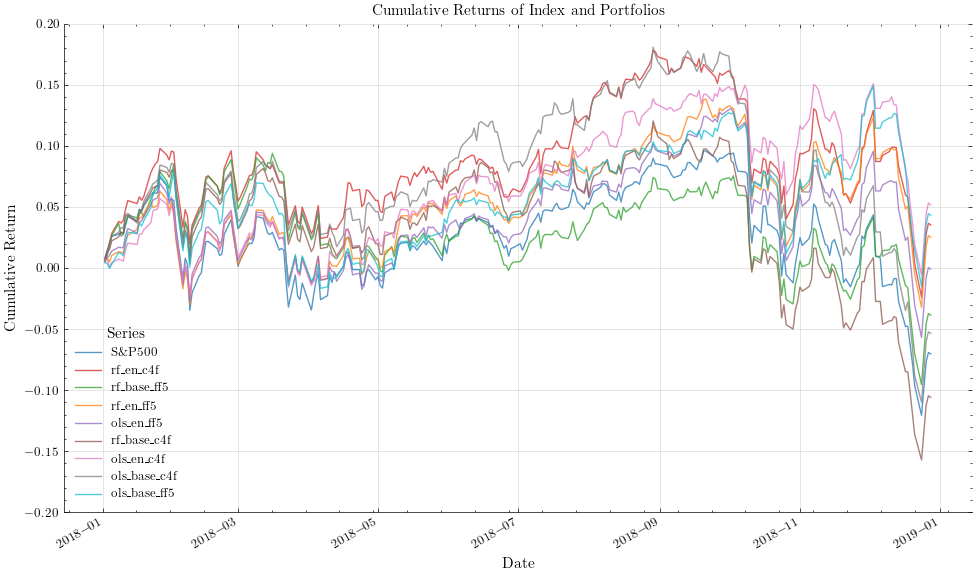
\includegraphics[width=\textwidth]{/Users/minhquangngo/Documents/vsc/erasmus/msc_thesis/latex/plots/results/cum_ret_plot.png}
    \caption{Cumulative returns of sector rotation strategies compared to S\&P500 index in 2018.}
    \label{fig:cum_ret_plot}
\end{figure}

- closer inspection of result however shows that for most of 2018, the S\&P500 index outperformed the sector rotation strategies.
- Surprsing that OLS baseline seems to keep up with the index from June to October (albeit a few percentage lower), while RF underperforms.